% Options for packages loaded elsewhere
\PassOptionsToPackage{unicode}{hyperref}
\PassOptionsToPackage{hyphens}{url}
%
\documentclass[
]{article}
\usepackage{lmodern}
\usepackage{amssymb,amsmath}
\usepackage{ifxetex,ifluatex}
\ifnum 0\ifxetex 1\fi\ifluatex 1\fi=0 % if pdftex
  \usepackage[T1]{fontenc}
  \usepackage[utf8]{inputenc}
  \usepackage{textcomp} % provide euro and other symbols
\else % if luatex or xetex
  \usepackage{unicode-math}
  \defaultfontfeatures{Scale=MatchLowercase}
  \defaultfontfeatures[\rmfamily]{Ligatures=TeX,Scale=1}
\fi
% Use upquote if available, for straight quotes in verbatim environments
\IfFileExists{upquote.sty}{\usepackage{upquote}}{}
\IfFileExists{microtype.sty}{% use microtype if available
  \usepackage[]{microtype}
  \UseMicrotypeSet[protrusion]{basicmath} % disable protrusion for tt fonts
}{}
\makeatletter
\@ifundefined{KOMAClassName}{% if non-KOMA class
  \IfFileExists{parskip.sty}{%
    \usepackage{parskip}
  }{% else
    \setlength{\parindent}{0pt}
    \setlength{\parskip}{6pt plus 2pt minus 1pt}}
}{% if KOMA class
  \KOMAoptions{parskip=half}}
\makeatother
\usepackage{xcolor}
\IfFileExists{xurl.sty}{\usepackage{xurl}}{} % add URL line breaks if available
\IfFileExists{bookmark.sty}{\usepackage{bookmark}}{\usepackage{hyperref}}
\hypersetup{
  pdftitle={Taller \# 3},
  pdfauthor={Julián Camilo Riaño Moreno},
  hidelinks,
  pdfcreator={LaTeX via pandoc}}
\urlstyle{same} % disable monospaced font for URLs
\usepackage[margin=1in]{geometry}
\usepackage{color}
\usepackage{fancyvrb}
\newcommand{\VerbBar}{|}
\newcommand{\VERB}{\Verb[commandchars=\\\{\}]}
\DefineVerbatimEnvironment{Highlighting}{Verbatim}{commandchars=\\\{\}}
% Add ',fontsize=\small' for more characters per line
\usepackage{framed}
\definecolor{shadecolor}{RGB}{248,248,248}
\newenvironment{Shaded}{\begin{snugshade}}{\end{snugshade}}
\newcommand{\AlertTok}[1]{\textcolor[rgb]{0.94,0.16,0.16}{#1}}
\newcommand{\AnnotationTok}[1]{\textcolor[rgb]{0.56,0.35,0.01}{\textbf{\textit{#1}}}}
\newcommand{\AttributeTok}[1]{\textcolor[rgb]{0.77,0.63,0.00}{#1}}
\newcommand{\BaseNTok}[1]{\textcolor[rgb]{0.00,0.00,0.81}{#1}}
\newcommand{\BuiltInTok}[1]{#1}
\newcommand{\CharTok}[1]{\textcolor[rgb]{0.31,0.60,0.02}{#1}}
\newcommand{\CommentTok}[1]{\textcolor[rgb]{0.56,0.35,0.01}{\textit{#1}}}
\newcommand{\CommentVarTok}[1]{\textcolor[rgb]{0.56,0.35,0.01}{\textbf{\textit{#1}}}}
\newcommand{\ConstantTok}[1]{\textcolor[rgb]{0.00,0.00,0.00}{#1}}
\newcommand{\ControlFlowTok}[1]{\textcolor[rgb]{0.13,0.29,0.53}{\textbf{#1}}}
\newcommand{\DataTypeTok}[1]{\textcolor[rgb]{0.13,0.29,0.53}{#1}}
\newcommand{\DecValTok}[1]{\textcolor[rgb]{0.00,0.00,0.81}{#1}}
\newcommand{\DocumentationTok}[1]{\textcolor[rgb]{0.56,0.35,0.01}{\textbf{\textit{#1}}}}
\newcommand{\ErrorTok}[1]{\textcolor[rgb]{0.64,0.00,0.00}{\textbf{#1}}}
\newcommand{\ExtensionTok}[1]{#1}
\newcommand{\FloatTok}[1]{\textcolor[rgb]{0.00,0.00,0.81}{#1}}
\newcommand{\FunctionTok}[1]{\textcolor[rgb]{0.00,0.00,0.00}{#1}}
\newcommand{\ImportTok}[1]{#1}
\newcommand{\InformationTok}[1]{\textcolor[rgb]{0.56,0.35,0.01}{\textbf{\textit{#1}}}}
\newcommand{\KeywordTok}[1]{\textcolor[rgb]{0.13,0.29,0.53}{\textbf{#1}}}
\newcommand{\NormalTok}[1]{#1}
\newcommand{\OperatorTok}[1]{\textcolor[rgb]{0.81,0.36,0.00}{\textbf{#1}}}
\newcommand{\OtherTok}[1]{\textcolor[rgb]{0.56,0.35,0.01}{#1}}
\newcommand{\PreprocessorTok}[1]{\textcolor[rgb]{0.56,0.35,0.01}{\textit{#1}}}
\newcommand{\RegionMarkerTok}[1]{#1}
\newcommand{\SpecialCharTok}[1]{\textcolor[rgb]{0.00,0.00,0.00}{#1}}
\newcommand{\SpecialStringTok}[1]{\textcolor[rgb]{0.31,0.60,0.02}{#1}}
\newcommand{\StringTok}[1]{\textcolor[rgb]{0.31,0.60,0.02}{#1}}
\newcommand{\VariableTok}[1]{\textcolor[rgb]{0.00,0.00,0.00}{#1}}
\newcommand{\VerbatimStringTok}[1]{\textcolor[rgb]{0.31,0.60,0.02}{#1}}
\newcommand{\WarningTok}[1]{\textcolor[rgb]{0.56,0.35,0.01}{\textbf{\textit{#1}}}}
\usepackage{longtable,booktabs}
% Correct order of tables after \paragraph or \subparagraph
\usepackage{etoolbox}
\makeatletter
\patchcmd\longtable{\par}{\if@noskipsec\mbox{}\fi\par}{}{}
\makeatother
% Allow footnotes in longtable head/foot
\IfFileExists{footnotehyper.sty}{\usepackage{footnotehyper}}{\usepackage{footnote}}
\makesavenoteenv{longtable}
\usepackage{graphicx,grffile}
\makeatletter
\def\maxwidth{\ifdim\Gin@nat@width>\linewidth\linewidth\else\Gin@nat@width\fi}
\def\maxheight{\ifdim\Gin@nat@height>\textheight\textheight\else\Gin@nat@height\fi}
\makeatother
% Scale images if necessary, so that they will not overflow the page
% margins by default, and it is still possible to overwrite the defaults
% using explicit options in \includegraphics[width, height, ...]{}
\setkeys{Gin}{width=\maxwidth,height=\maxheight,keepaspectratio}
% Set default figure placement to htbp
\makeatletter
\def\fps@figure{htbp}
\makeatother
\setlength{\emergencystretch}{3em} % prevent overfull lines
\providecommand{\tightlist}{%
  \setlength{\itemsep}{0pt}\setlength{\parskip}{0pt}}
\setcounter{secnumdepth}{-\maxdimen} % remove section numbering
\usepackage{float}
\floatplacement{figure}{H}
\usepackage{subfig}
\usepackage{graphicx}

\title{Taller \# 3}
\usepackage{etoolbox}
\makeatletter
\providecommand{\subtitle}[1]{% add subtitle to \maketitle
  \apptocmd{\@title}{\par {\large #1 \par}}{}{}
}
\makeatother
\subtitle{Ejericicio regresión logística}
\author{Julián Camilo Riaño Moreno}
\date{miércoles, abril 08, 2020}

\begin{document}
\maketitle

{
\setcounter{tocdepth}{3}
\tableofcontents
}
\pagebreak

\hypertarget{descripciuxf3n-de-las-variables.}{%
\section{Descripción de las
variables.}\label{descripciuxf3n-de-las-variables.}}

\begin{longtable}[]{@{}cccccc@{}}
\caption{Organizacion de las variables del taller \#4}\tabularnewline
\toprule
\begin{minipage}[b]{0.07\columnwidth}\centering
Modelo\strut
\end{minipage} & \begin{minipage}[b]{0.13\columnwidth}\centering
Definicion\strut
\end{minipage} & \begin{minipage}[b]{0.17\columnwidth}\centering
Tipo de variable (en modelo)\strut
\end{minipage} & \begin{minipage}[b]{0.18\columnwidth}\centering
Nombre de variable (en la base de datos)\strut
\end{minipage} & \begin{minipage}[b]{0.15\columnwidth}\centering
Unidad\strut
\end{minipage} & \begin{minipage}[b]{0.13\columnwidth}\centering
Tipo de variable\strut
\end{minipage}\tabularnewline
\midrule
\endfirsthead
\toprule
\begin{minipage}[b]{0.07\columnwidth}\centering
Modelo\strut
\end{minipage} & \begin{minipage}[b]{0.13\columnwidth}\centering
Definicion\strut
\end{minipage} & \begin{minipage}[b]{0.17\columnwidth}\centering
Tipo de variable (en modelo)\strut
\end{minipage} & \begin{minipage}[b]{0.18\columnwidth}\centering
Nombre de variable (en la base de datos)\strut
\end{minipage} & \begin{minipage}[b]{0.15\columnwidth}\centering
Unidad\strut
\end{minipage} & \begin{minipage}[b]{0.13\columnwidth}\centering
Tipo de variable\strut
\end{minipage}\tabularnewline
\midrule
\endhead
\begin{minipage}[t]{0.07\columnwidth}\centering
\(\beta_0\)\strut
\end{minipage} & \begin{minipage}[t]{0.13\columnwidth}\centering
Presenta dengue\strut
\end{minipage} & \begin{minipage}[t]{0.17\columnwidth}\centering
v\_respuesta\strut
\end{minipage} & \begin{minipage}[t]{0.18\columnwidth}\centering
enf\_dengue\strut
\end{minipage} & \begin{minipage}[t]{0.15\columnwidth}\centering
1 = si; 0 = No\strut
\end{minipage} & \begin{minipage}[t]{0.13\columnwidth}\centering
Categorica binomial\strut
\end{minipage}\tabularnewline
\begin{minipage}[t]{0.07\columnwidth}\centering
\(\beta_1\)\strut
\end{minipage} & \begin{minipage}[t]{0.13\columnwidth}\centering
Edad\strut
\end{minipage} & \begin{minipage}[t]{0.17\columnwidth}\centering
v\_regresora\strut
\end{minipage} & \begin{minipage}[t]{0.18\columnwidth}\centering
edad\strut
\end{minipage} & \begin{minipage}[t]{0.15\columnwidth}\centering
Anos\strut
\end{minipage} & \begin{minipage}[t]{0.13\columnwidth}\centering
Cuantitativa distreta\strut
\end{minipage}\tabularnewline
\begin{minipage}[t]{0.07\columnwidth}\centering
\(\beta_2\)\strut
\end{minipage} & \begin{minipage}[t]{0.13\columnwidth}\centering
Nivel socioeconomico\strut
\end{minipage} & \begin{minipage}[t]{0.17\columnwidth}\centering
v\_regresora\strut
\end{minipage} & \begin{minipage}[t]{0.18\columnwidth}\centering
nivel\_soc\_econ\strut
\end{minipage} & \begin{minipage}[t]{0.15\columnwidth}\centering
1 = nivel alto; 2 = nivel medio; 3 = nivel bajo\strut
\end{minipage} & \begin{minipage}[t]{0.13\columnwidth}\centering
Categorica ordinal\strut
\end{minipage}\tabularnewline
\begin{minipage}[t]{0.07\columnwidth}\centering
\(\beta_3\)\strut
\end{minipage} & \begin{minipage}[t]{0.13\columnwidth}\centering
Sector en el que vive\strut
\end{minipage} & \begin{minipage}[t]{0.17\columnwidth}\centering
v\_regresora\strut
\end{minipage} & \begin{minipage}[t]{0.18\columnwidth}\centering
sector\_vive\strut
\end{minipage} & \begin{minipage}[t]{0.15\columnwidth}\centering
Sector = 1 o 2\strut
\end{minipage} & \begin{minipage}[t]{0.13\columnwidth}\centering
Categorica nominal\strut
\end{minipage}\tabularnewline
\bottomrule
\end{longtable}

\hypertarget{respuesta-a-la-preguntas-del-taller-4}{%
\section{Respuesta a la preguntas del taller \#
4}\label{respuesta-a-la-preguntas-del-taller-4}}

\hypertarget{problema}{%
\subsection{Problema}\label{problema}}

En un estudio para investigar la incidencia de dengue en una determinada
ciudad de la costa mexicana, un total de 196 individuos, escogidos
aleatoriamente en dos de los sectores de la ciudad, respondió a las
siguientes preguntas: (i) (edad) Edad (en a\textasciitilde nos), (ii)
(nivel) nivel socioeconómico (1 nivel alto/ 2 nivel medio/ 3 nivel
bajo), (iii) (sector) sector en el que vive y (iv) (enfermedad) si el
entrevistado contrajo o no la enfermedad recientemente (1 si/ 0 no).

\hypertarget{pregunta-1-considere-un-modelo-loguxedstico-lineal-para-explicar-la-probabilidad-de-que-un-individuo-contraiga-la-enfermedad-a-partir-de-las-tres-variables-explicativas.-describa-las-componentes-aleatoria-y-sistemuxe1tica-del-modelo-propuesto.}{%
\subsubsection{Pregunta \#1: Considere un modelo logístico lineal para
explicar la probabilidad de que un individuo contraiga la enfermedad a
partir de las tres variables explicativas. Describa las componentes
aleatoria y sistemática del modelo
propuesto.}\label{pregunta-1-considere-un-modelo-loguxedstico-lineal-para-explicar-la-probabilidad-de-que-un-individuo-contraiga-la-enfermedad-a-partir-de-las-tres-variables-explicativas.-describa-las-componentes-aleatoria-y-sistemuxe1tica-del-modelo-propuesto.}}

\begin{itemize}
\tightlist
\item
  Componentes aleatoria: corresponde a la variable respuesta
  \texttt{enf\_dengue}. Como está descrito en la tabla 1. Es una
  variables categórica dicotómica o binomia, que puede tomar el valor 1
  cuando el caso tiene la enfermedad del dengue o valor 0 cuando no la
  tiene.
\item
  Compoenentes sistemática: corresponde a las tres variables regresoras
  \texttt{edad}, \texttt{nivel\_soc\_econ}, \texttt{sec\_vive}. Las
  especificaciones acerca de la unidad de medida y el tipo de variable
  está descrito en la tabla 1.
\item
  Función enlace o función \(logit\): \(\ln \frac{\pi}{\pi - 1}\)
\end{itemize}

\begin{longtable}[]{@{}lrrrr@{}}
\caption{Estimadores, \(z-values\), \(p-values\) del modelo de regresión
logística}\tabularnewline
\toprule
& Estimado & ErrorStand & \(z-value\) & \(p-value\)\tabularnewline
\midrule
\endfirsthead
\toprule
& Estimado & ErrorStand & \(z-value\) & \(p-value\)\tabularnewline
\midrule
\endhead
(Intercept) & -2.2939 & 0.4368 & -5.2521 & 0.0000\tabularnewline
edad & 0.0270 & 0.0087 & 3.1114 & 0.0019\tabularnewline
factor(nivel\_soc\_econ)2 & 0.0446 & 0.4325 & 0.1031 &
0.9178\tabularnewline
factor(nivel\_soc\_econ)3 & 0.2534 & 0.4055 & 0.6249 &
0.5320\tabularnewline
factor(sector\_vive)2 & 1.2436 & 0.3523 & 3.5303 & 0.0004\tabularnewline
\bottomrule
\end{longtable}

La tabla 2. muestra los estimadores obtenidos por el modelo logistico
aplicado. Allí se puede observar que tan solo las variables regresoras
\texttt{edad}y \texttt{sector\_vive}son significativas
(\(p - value < 0.05\)) y por lo tanto son suceptibles de interpretación.
El nivel socio económico en niguno de sus niveles (1, 2, o 3) tienen
significancia.

\begin{longtable}[]{@{}cccc@{}}
\caption{Tests de bondad de ajuste del modelo: Pseudo \(R^2\) de
McFadden (ps-\(R^2\)) \& Test de Hosmer-Lemeshow (\(ji^2\)
HL)}\tabularnewline
\toprule
ps-\(R^2\) & \(ji^2\) HL & G.libertad (\(ji^2\) HL) &
\(p-value(ji^2 HL)\)\tabularnewline
\midrule
\endfirsthead
\toprule
ps-\(R^2\) & \(ji^2\) HL & G.libertad (\(ji^2\) HL) &
\(p-value(ji^2 HL)\)\tabularnewline
\midrule
\endhead
0.1062 & 8.0633 & 8 & 0.4273\tabularnewline
\bottomrule
\end{longtable}

Para evaluar la bondad del modelo aplicado ser realizó dos pruebas de
bodad de ajuste (tabla 3). En primer lugar, se llevo acabo un
pseudo-\(R^2\) de McFadden con un resultado de 0.106 si este valor rodea
0.2 a 0.4 quiere decir buen ajuste\footnote{Domencich \& McFadden (1975)
  Urban Travel Demand: A Behavioral Analysis, Elsevier.}. Según lo
anterior el estadístico de McFadden no muestra buen ajuste del modelo.

En la misma tabla 3. se encuentra el resultado del test de
Hosmer-Lemeshow, es cual establece que \(H_0\) = buen ajuste del modelo
y \(H_1 =\) modelo no tiene buen ajuste. Este ajuste se da através de
las diferencias entre los valores observados y los valores esperados
predichos por el modelo, entonces \(H_0\) = indica que no hay
diferencias significativas entre los valores observados y los esperados
y \(H_1 =\) que existen diferencias significativas.

\begin{figure}
\centering
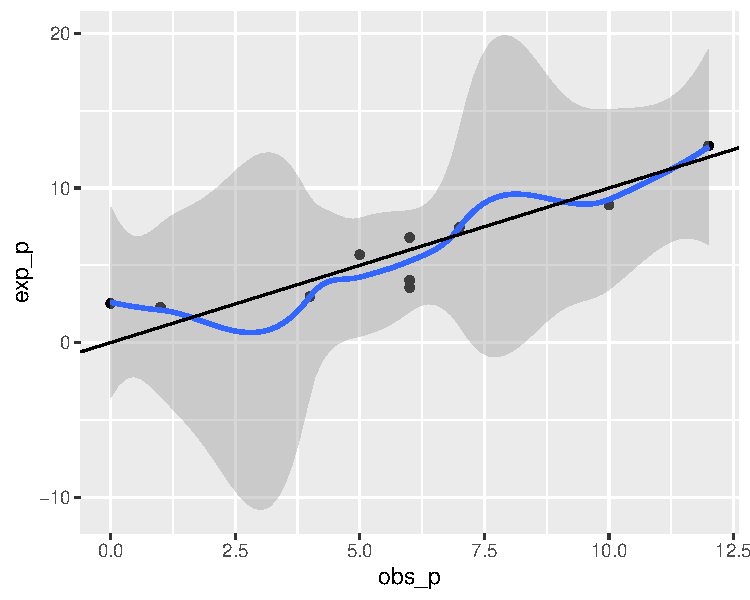
\includegraphics{taller4_regresionlogist_files/figure-latex/gráfica de relación de esperados y observados Hosmer-lemeshow-1.pdf}
\caption{Relación esperados vs observados en un modelo probado por test
Hosmer-Lemeshow}
\end{figure}

Como se puede observar en la tabla 3. El test de Hosmer-Lemeshow no es
significativo (\(p - value = 0.4273, \geq 0.05\)). De manera que no se
puede rechazar la hipotesis nula y se puede concluir que el modelo tiene
buen ajuste. La figura 1. muestra la relación entre los valores
observados y esperados por el modelo. La curva azul es la curva de
correlación y la negra corresponde a una correlación exacta. De esto se
puede concluir que la relación entre las diferencias de los valores
observados y esperados giran entorno la linea de referencia por lo tanto
sus defencias no son muy grandes.

\begin{longtable}[]{@{}cccc@{}}
\caption{Comparación Deviance NULL vs Deviance del modelo
LOGIT}\tabularnewline
\toprule
Deviance\_NULL (DN) & G.libertad (DN) & Deviance\_modelo (DM) &
G.libertad(DM)\tabularnewline
\midrule
\endfirsthead
\toprule
Deviance\_NULL (DN) & G.libertad (DN) & Deviance\_modelo (DM) &
G.libertad(DM)\tabularnewline
\midrule
\endhead
236.3293 & 195 & 211.22 & 191\tabularnewline
\bottomrule
\end{longtable}

Finalmente se realizó un análisis de \emph{Deviance} los cuales servir
como indicadores de \emph{maldad} y ajuste del modelo. En la tabla 4 se
muestra el valor del \emph{deviance} en un modelo sin variables
regresoras (NULL) con un resultado de 263.33 y el valor del
\emph{deviance} en el modelo logístico resultado para las variables
dadas con un resultado de 211.22. En este caso se asume que si el
\emph{deviance} del modelo es menor que el \emph{deviance} NULL, el
modelo tiene mejor ajuste, lo que es verdadero para este caso.

\begin{longtable}[]{@{}lcc@{}}
\caption{Exponencial razón de odds \(e^{coeff}\)}\tabularnewline
\toprule
& \(e^{coeff} = \pi\) & \((\pi-1)\times100 (\%)\)\tabularnewline
\midrule
\endfirsthead
\toprule
& \(e^{coeff} = \pi\) & \((\pi-1)\times100 (\%)\)\tabularnewline
\midrule
\endhead
(Intercept) & 0.1009 & 89.9131\tabularnewline
edad & 1.0274 & 2.7359\tabularnewline
factor(nivel\_soc\_econ)2 & 1.0456 & 4.5619\tabularnewline
factor(nivel\_soc\_econ)3 & 1.2884 & 28.8441\tabularnewline
factor(sector\_vive)2 & 3.4682 & 246.8181\tabularnewline
\bottomrule
\end{longtable}

\hypertarget{pregunta-2-la-probabilidad-de-que-un-individuo-contraiga-la-enfermedad-depende-de-su-edad}{%
\subsubsection{Pregunta \#2: La probabilidad de que un individuo
contraiga la enfermedad depende de su
edad?}\label{pregunta-2-la-probabilidad-de-que-un-individuo-contraiga-la-enfermedad-depende-de-su-edad}}

El análisis de los estimadores los \(z-value\) y sus correspondientes
\(p-values\) evidenciados en la tabla 2, se podría afirmar que la
variable \texttt{edad} si puede afectar el \(\beta_0\) (tener la
enfermedad dengue o la variable respuesta \texttt{enf\_dengue}). En este
caso se podría afirmar que por cada incremento en una unidad de
\texttt{edad} el chance de tener Dengue incrementa en un 2.73\% como se
puede ver en la tabla 5.

\hypertarget{pregunta-3-la-probabilidad-de-que-un-individuo-contraiga-la-enfermedad-depende-del-sector-de-la-ciudad-en-el-que-vive}{%
\subsubsection{Pregunta \#3: La probabilidad de que un individuo
contraiga la enfermedad depende del sector de la ciudad en el que
vive?}\label{pregunta-3-la-probabilidad-de-que-un-individuo-contraiga-la-enfermedad-depende-del-sector-de-la-ciudad-en-el-que-vive}}

En este caso a través de los resultados mostrados en la tabla 2, se
podría afirmar que la variable \texttt{sector\_vive} si puede afectar el
\(\beta_0\) (tener la enfermedad dengue o la variable respuesta
\texttt{enf\_dengue}). En este caso se podría afirmar que el vivir en el
sector 2 incrementa el 243\% el chance de tener Dengue respecto a vivir
en el sector 1 como se puede ver en los resultados de la tabla 5.

\hypertarget{pregunta-4-seguxfan-el-modelo-estimado-cuuxe1l-es-la-probabilidad-de-contraer-dengue-de-una-persona-de-30-auxf1oos-nivel-socioeconuxf3mico-alto-y-que-vive-en-el-sector-2-de-la-ciudad}{%
\subsubsection{Pregunta \#4: Según el modelo estimado, cuál es la
probabilidad de contraer dengue de una persona de 30 añoos, nivel
socioeconómico alto y que vive en el sector 2 de la
ciudad?}\label{pregunta-4-seguxfan-el-modelo-estimado-cuuxe1l-es-la-probabilidad-de-contraer-dengue-de-una-persona-de-30-auxf1oos-nivel-socioeconuxf3mico-alto-y-que-vive-en-el-sector-2-de-la-ciudad}}

\begin{Shaded}
\begin{Highlighting}[]
\KeywordTok{predict}\NormalTok{(denguelogit, }\KeywordTok{data.frame}\NormalTok{(}\DataTypeTok{sector_vive=}\DecValTok{2}\NormalTok{, }\DataTypeTok{nivel_soc_econ=}\DecValTok{1}\NormalTok{,}\DataTypeTok{edad=}\DecValTok{30}\NormalTok{), }\DataTypeTok{type=}\StringTok{"response"}\NormalTok{)}
\end{Highlighting}
\end{Shaded}

Para dar respuesta a la pregunta 4 como se puede ver se hizo uso de la
función \texttt{predict}. Definiendo los paramétros solicitados, se
obtiene que, a traés del modelo \emph{logit} realizado la probabilidad
de contraer la enfermedad por Dengue en una persona de 30 años que viva
en el sector 2 y que sea de nivel socioeconómico alto es del 44\%.

\hypertarget{pregunta-5-seleccione-el-mejor-modelo-para-describir-el-fenuxf3meno-bajo-estudio.-use-como-guuxeda-la-medida-de-calidad-del-ajuste-aic.-verifuxedque-que-todas-las-variables-en-el-modelo-elegido-sean-estaduxedsticamente-signifuxedcativas.-interprete-los-paruxe1metros-del-modelo-escogido.}{%
\subsubsection{Pregunta \#5: Seleccione el ``mejor'' modelo para
describir el fenómeno bajo estudio. Use como guía la medida de calidad
del ajuste AIC. Verifíque que todas las variables en el modelo elegido
sean estadísticamente signifícativas. INTERPRETE los parámetros del
modelo
escogido.}\label{pregunta-5-seleccione-el-mejor-modelo-para-describir-el-fenuxf3meno-bajo-estudio.-use-como-guuxeda-la-medida-de-calidad-del-ajuste-aic.-verifuxedque-que-todas-las-variables-en-el-modelo-elegido-sean-estaduxedsticamente-signifuxedcativas.-interprete-los-paruxe1metros-del-modelo-escogido.}}

\begin{Shaded}
\begin{Highlighting}[]
\KeywordTok{step}\NormalTok{(}\DataTypeTok{object =}\NormalTok{ Full_denguelogit, }\DataTypeTok{direction =} \StringTok{"both"}\NormalTok{, }\DataTypeTok{trace =} \OtherTok{FALSE}\NormalTok{)}
\end{Highlighting}
\end{Shaded}

Para realizar la selección del mejor modelo se utilizo una estrategía
\emph{stepwise} bidireccional \footnote{Se intentó un \emph{stepwise}
  unidireccional \emph{forward} como se encontraba en el script
  facilitado por el profesor, pero se encontró que bajo esta estrategía
  el resultado era el mismo que el modelo original, con la variable
  \texttt{nivel\_soc\_econ}no significativa. Al utiliza el método
  bidireccional se garantizó que todas las variables fueran
  estadísticamente significativas.} (forward y reverse, parametro
\texttt{both}), a través de la función \texttt{step}. Su resultado
permitió establecer como ``mejor modelo'' (como se designara en
adelante), de únicamente dos variables regresoras \texttt{edad} y
\texttt{sec\_vive}, excluyendo la variables no siginificativas en el
modelo original \texttt{nivel\_soc\_econ} 2 y 3. Como se puede observar
en la tabla 6 el AIC del mejor modelo es menor que el AIC el modelo
original, lo que corrobora al primero como ``mejor'', para las variables
dadas. De esta forma, los análisis a continuación se realizarán con este
``mejor modelo'' de dos variables regresoras.

\begin{longtable}[]{@{}cc@{}}
\caption{Comparación de valor AIC del modelo original y el mejor modelo
obtenido por el estadítico}\tabularnewline
\toprule
AIC\_modelo\_original & AIC\_mejor\_modelo\tabularnewline
\midrule
\endfirsthead
\toprule
AIC\_modelo\_original & AIC\_mejor\_modelo\tabularnewline
\midrule
\endhead
221.22 & 217.6393\tabularnewline
\bottomrule
\end{longtable}

La tabla 7, muestra los estimadores del mejor modelo con sus respectivos
\(z-value\) y \(p-value\) como se puede observar en este caso todas las
variables son significativas estadísticamente (\(p-value < 0.05\)).

\begin{longtable}[]{@{}lrrrr@{}}
\caption{Estimadores, \(z-values\), \(p-values\) del mejor modelo de
regresión logística}\tabularnewline
\toprule
& Estimado & ErrorStand & \(z-value\) & \(p-value\)\tabularnewline
\midrule
\endfirsthead
\toprule
& Estimado & ErrorStand & \(z-value\) & \(p-value\)\tabularnewline
\midrule
\endhead
(Intercept) & -2.1597 & 0.3439 & -6.2802 & 3.381506e-10\tabularnewline
edad & 0.0268 & 0.0086 & 3.0998 & 1.936226e-03\tabularnewline
factor(sector\_vive)2 & 1.1817 & 0.3370 & 3.5070 &
4.532196e-04\tabularnewline
\bottomrule
\end{longtable}

\begin{longtable}[]{@{}cccc@{}}
\caption{Tests de bondad de ajuste del mejor modelo: Pseudo \(R^2\) de
McFadden (ps-\(R^2\)) \& Test de Hosmer-Lemeshow (\(ji^2\)
HL)}\tabularnewline
\toprule
ps-\(R^2\) & \(ji^2\) HL & G.libertad (\(ji^2\) HL) &
\(p-value(ji^2 HL)\)\tabularnewline
\midrule
\endfirsthead
\toprule
ps-\(R^2\) & \(ji^2\) HL & G.libertad (\(ji^2\) HL) &
\(p-value(ji^2 HL)\)\tabularnewline
\midrule
\endhead
0.1045 & 14.9561 & 8 & 0.06\tabularnewline
\bottomrule
\end{longtable}

Al igual que con el modelo original, se realizaron para el mejor modelo
las pruebas de bondad de pseudo \(R^2\) de McFadden y el test de
Hosmer-Lemeshow. Sus resultados pueden econtrarse en la tabla 8. Allí se
evidencia que la valoración por el primer estadístico permanece en 0.10
lo que sugiere que el modelo no tiene buen ajuste. Sin embargo, el
segundo estadístico muestra un \(p-value < 0.05\) de manera que no se
puede rechazar la hipotesis nula (\(H_0\)), y se puede considerar en
este caso que el mejor modelo tiene buen ajuste dado que los valores
esperados predichos por el modelo no se diferencia significativamente de
los observados. Este hecho puede verse en la figura 2, sin embargo, allí
se puede encontrar un mayor distanciamiento de la linea de correlación
(azul) de la linea de referencia, que lo observado en el modelo
original.

\begin{figure}
\centering
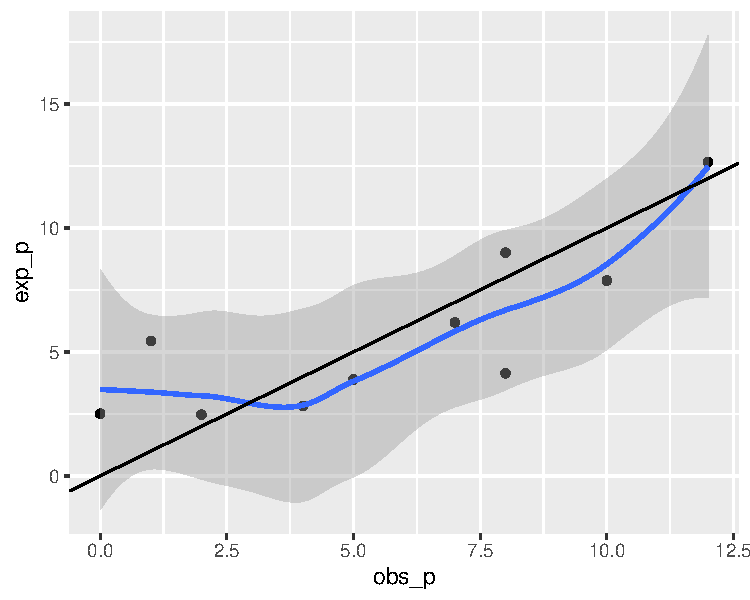
\includegraphics{taller4_regresionlogist_files/figure-latex/gráfica de relación de esperados y observados MEJOR MODELO Hosmer-lemeshow-1.pdf}
\caption{Relación esperados vs observados para mejor modelo probado por
test Hosmer-Lemeshow}
\end{figure}

Finalmente se realizó una comparación de \emph{Deviance} del mejor
modelo, los resultados se pueden encontrar en la tabla 9. Donde al igual
que el modelo original, el valor del \emph{deviance} del modelo es menor
que el valor del \emph{deviance} sin variable regresoras (NULL), lo que
comprueba un buen ajuste en el mejor modelo.

\begin{longtable}[]{@{}cccc@{}}
\caption{Comparación Deviance NULL vs Deviance del mejor modelo
LOGIT}\tabularnewline
\toprule
Deviance\_NULL (DN) & G.libertad (DN) & Deviance\_modelo (DM) &
G.libertad(DM)\tabularnewline
\midrule
\endfirsthead
\toprule
Deviance\_NULL (DN) & G.libertad (DN) & Deviance\_modelo (DM) &
G.libertad(DM)\tabularnewline
\midrule
\endhead
236.3293 & 195 & 211.6393 & 193\tabularnewline
\bottomrule
\end{longtable}

\hypertarget{pregunta-6-describa-el-desempeuxf1o-del-modelo-seleccionado-usando-su-matriz-de-confusiuxf3n.}{%
\subsubsection{Pregunta \#6: Describa el desempeño del modelo
seleccionado usando su matriz de
confusión.}\label{pregunta-6-describa-el-desempeuxf1o-del-modelo-seleccionado-usando-su-matriz-de-confusiuxf3n.}}

Las tablas 10 y 11 corresponden a las tablas de confusión para el modelo
original y el mejor modelo respectivamente. Como se puede observar el
mejor modelo presenta menor error tipo 1 (falsos negativos) (41 vs 40).
Por otra parte, se realizó el análisis de \emph{Accuracy} (o exactitud)
encontrandose que el mejor modelo tiene 75\% de probabilidades de
encontrar personas enfermas con Dengue, mientras el modelo original
tiene un 74\%. De esta forma se concluye que el mejor modelo, es más
preciso que el original y de esté es posible realizar mejore
interpretaciones.

\begin{longtable}[]{@{}lcc@{}}
\caption{Matriz de confusión para el modelo original}\tabularnewline
\toprule
& FALSE & TRUE\tabularnewline
\midrule
\endfirsthead
\toprule
& FALSE & TRUE\tabularnewline
\midrule
\endhead
0 & 130 & 9\tabularnewline
1 & 41 & 16\tabularnewline
\bottomrule
\end{longtable}

\begin{longtable}[]{@{}lcc@{}}
\caption{Matriz de confusion para el mejor modelo}\tabularnewline
\toprule
& FALSE & TRUE\tabularnewline
\midrule
\endfirsthead
\toprule
& FALSE & TRUE\tabularnewline
\midrule
\endhead
0 & 130 & 9\tabularnewline
1 & 40 & 17\tabularnewline
\bottomrule
\end{longtable}

\begin{longtable}[]{@{}cc@{}}
\caption{Comparación \emph{Accuracy} del modelo original Vs mejor
modelo}\tabularnewline
\toprule
Accuraccy Modelo\_original & Accuracy Mejor\_Modelo\tabularnewline
\midrule
\endfirsthead
\toprule
Accuraccy Modelo\_original & Accuracy Mejor\_Modelo\tabularnewline
\midrule
\endhead
0.7449 & 0.75\tabularnewline
\bottomrule
\end{longtable}

\end{document}
